%Speed-Ding

\begin{figure}[h!]
\begin{center}
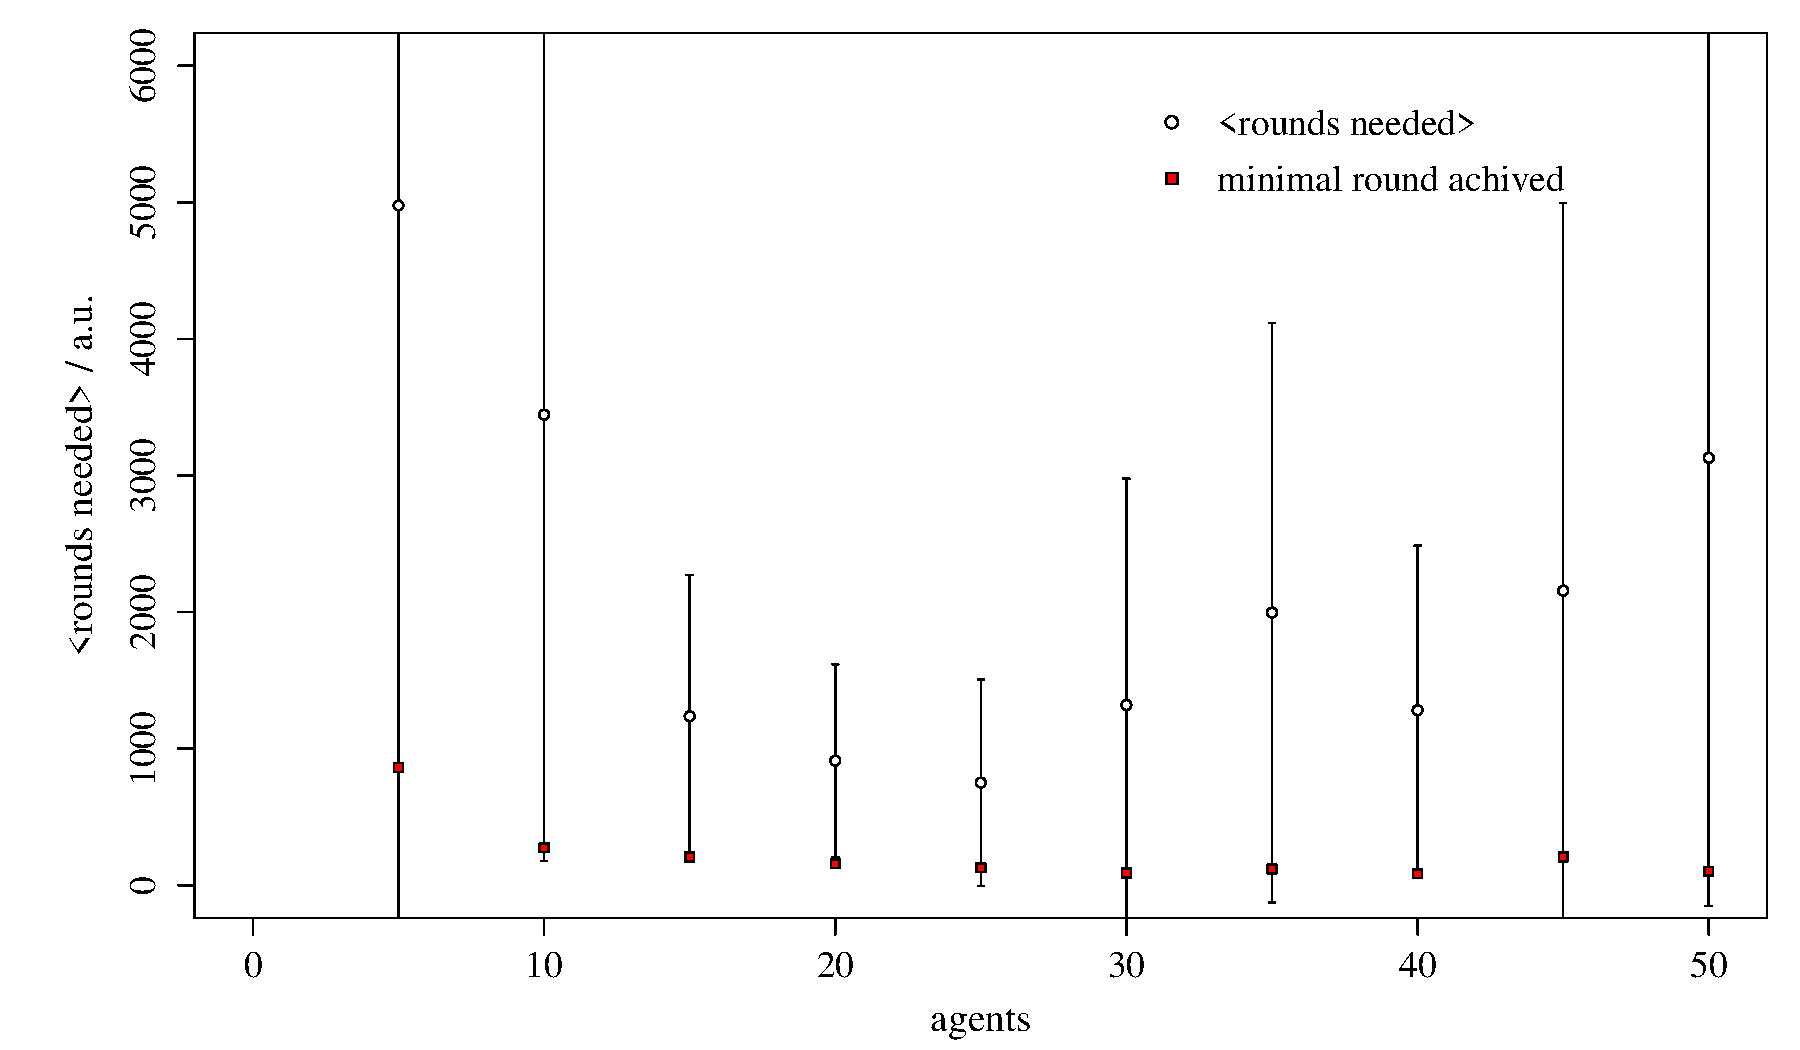
\includegraphics[width=0.9\linewidth]{rounds_needed_average_vs_shortestpath}
\caption{To determine after how many rounds the shortest path is definitely found the program is adapted such that the for-loop over the number of rounds is replaced by a while loop. When the optimal tour length, known form previous calculations, is achieved three times in series the while loop is left. This plot shows the number of rounds needed to fulfill this criteria for different ant colony sizes. The values are averaged over ten runs and show a large spread. The bigger the error bars the more possible it is for agents to get stuck in a local minimal which does not correspond to the optimal tour. But due to the big uncertainties no direct correlation between the average time needed to find the shortest path and the number of agents can be made. However, the smallest number of rounds needed to find the solution in ten trials decreases for more than five agents.}
\label{fig:speed}
\end{center}
\end{figure}